\documentclass{article}

\usepackage{geometry}
\usepackage{graphicx}
\usepackage{nopageno}
\usepackage{tikz}
\usepackage{float}
\usetikzlibrary{shapes.callouts}

\title{TODO: Title}
\author{Anonymous Authors}
\date{}

\begin{document}
\maketitle

\section{Introduction}

The aim of this paper is to bring peace! For years very smart people have been
fighting over the shape of our beautiful, albeit shitty, planet. Two equally
reasonable positions have mainly emerged: the Earth is a disc VS the Earth is a
sphere. This two very different bidimensional manifolds have both equal rights
to claim themselves the proper geometrical model for Earth. Thus they started
fighting. With what army? Well, Flat Earth Societies are fighting in the blue
corner alongside the multiple-millenia champion Disc. In the red corner we see
the young arrogant opponent, the Sphere, supported by its team: Science and
everyone else.

They have been fighting round after round for centuries, with equal
credibility, and the match seemed impossible to settle. There was this dark
moment in history where the evil and arrogant was unfairly holding our beloved
champion against the ropes. All seemed lost. How can planes fly in
circonferences around the globe if the globe is not a globe? That was a tough
one, also a shitty move in the authors' opinion. Then Pacman, the fairest
referee of all, came to save the day.

The main contribution of this work is none. However, we would like to remind
everyone that the Pacman effect is a thing. Airplanes can fly to the extreme
boundary of Earth, but they are bound to reappear on the diametrically opposite
side of the disc, just like Pacman in the famous Namco videogame. Now when
forced to apply the rigour of mathematics (reluctantly: reasoning is for nerds!
Nerds suck!), we see that the Pacman effect can be modelled as the
identification of the boundary of the disc to one single point.

Counterintuitively this Pacman effect sheds new light on the Truth. The disc
with such identified border is nothing but a surface diffeomorph to the sphere.
As Einstein once said:

``It seems as though we must use sometimes the one theory and sometimes the
other, while at times we may use either. We are faced with a new kind of
difficulty. We have two contradictory pictures of reality; separately neither
of them fully explains the phenomena of light [L to All: I would strike on the
word ``light'' and write Earth next to it], but together they do.''

We have discovered what we call the ``disc–sphere duality''.

\begin{figure}[ht]
  \centering
  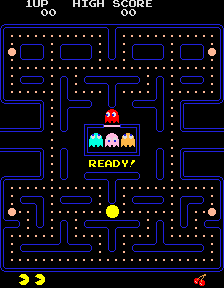
\includegraphics{images/pacman.png}
  \caption{A Screenshot of Pacman}
  \label{fig:pacman-screenshot}
\end{figure}

\section{Flat and spherical earth are very different views of the world}
\section{Pacman says: ``Are they though?''}
\begin{figure}[H]
  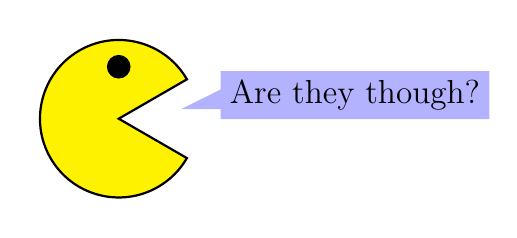
\begin{tikzpicture}
    % https://tex.stackexchange.com/questions/428967/pacman-circle-in-tikz
    \draw[thick,fill=yellow]
      (0,0) -- (30:1cm) arc (30:330:1cm) -- cycle;
    \fill (0,0.66) circle (1.5mm);
    \node[rectangle callout, callout relative pointer={(-0.5cm,-0.04cm)},
        fill=blue!30] at (3,0.3) {\large Are they though?};
  \end{tikzpicture}
\end{figure}
\section{No they aren't}
\section{Conclusion and Future Work}

\end{document}
